\documentclass[12pt]{article}
\usepackage[a4paper, margin=2.54cm, headheight=14pt]{geometry}
\usepackage{setspace}
\usepackage{times}
\usepackage{amsmath, amssymb}
\usepackage{booktabs}
\usepackage{array}
\usepackage{graphicx}
\usepackage{hyperref}
\usepackage[authoryear,round]{natbib}
\usepackage{fancyhdr}
\usepackage{titlesec}
\usepackage{microtype}
\usepackage[T1]{fontenc}
\usepackage[utf8]{inputenc}
\usepackage{caption}
\usepackage{float}
\usepackage[section]{placeins}

\doublespacing
\setlength{\parindent}{0.5in}
\setlength{\parskip}{0pt}
\pagestyle{fancy}
\fancyhf{}
\rhead{\small\MakeUppercase{Supporting Information}}
\rfoot{S\thepage}
\renewcommand{\headrulewidth}{0pt}
\titleformat{\section}{\normalfont\normalsize\bfseries}{\thesection.}{0.5em}{}
\titleformat{\paragraph}[runin]{\normalfont\normalsize\bfseries}{}{0pt}{}[\ ---]
\titlespacing*{\paragraph}{0pt}{6pt}{0.5em}
\hypersetup{colorlinks=true, linkcolor=blue, citecolor=blue, urlcolor=blue,
  pdftitle={Supporting Information: Null-Model Choice for Rule-Defined Pattern Counts in Clustered Longitudinal Sequences: A Case Study of Jewish Halachic Menstrual Anticipation Rules},
  pdfauthor={Dvir Ross}}
\newcolumntype{L}[1]{>{\raggedright\arraybackslash}p{#1}}
\newcolumntype{C}[1]{>{\centering\arraybackslash}p{#1}}
\graphicspath{{figures/}}
\captionsetup{font=small, labelfont=bf, width=0.92\textwidth}
\renewcommand{\thesection}{S\arabic{section}}
\renewcommand{\thetable}{S\arabic{table}}
\renewcommand{\thefigure}{S\arabic{figure}}
\newcommand{\HG}{H_{G}}
\newcommand{\HI}{H_{iid}}
\newcommand{\HW}{H_{W}}
\providecommand{\doi}{}
\renewcommand{\doi}[1]{\href{https://doi.org/#1}{\nolinkurl{https://doi.org/#1}}}

\begin{document}

\begin{center}
{\large\bfseries Supporting Information}\\[6pt]
{\normalsize Null-Model Choice for Rule-Defined Pattern Counts in Clustered Longitudinal
Sequences: A Case Study of Jewish Halachic Menstrual Anticipation Rules}\\[4pt]
{\normalsize Dvir Ross}
\end{center}

\bigskip
\noindent This document contains the exploratory between-woman pairwise dependence
analysis referred to in Sections~3.4, 4.4 and 5.2 of the main article (Section~S1), the
literature search referred to in Section~1 (Section~S2) and the evaluation of the
zero-count rule \textit{Haflaga Chozer Chalila} referred to in Sections~2.1 and 3.1
(Section~S3). The pairwise analysis is
secondary to the null-model comparison and does not bear on the primary question of
whether within-woman ordering produces excess rule-defined events. Notation follows the
main article; all computations are produced by \texttt{scripts/postprocess.py} and the
accompanying notebook in the code repository
(\url{https://github.com/dvirross/VessetVectorTest}).

\medskip
\noindent The SHA-256 checksum of the released filtered data file
(\nolinkurl{data/FilteredData.csv}; 1,554 cycles, 118 women), for verifying file
integrity, is
\begin{center}
\small\texttt{508ee88efb18bcd29c7ed6f841827377bb8d72a8c7dd38fdeb40cf08691f7811}
\end{center}

\section{Exploratory Pairwise Dependence Between Pattern Types}
\label{sec:si-pairwise}

\subsection*{S1.1 Question and expectations}

The joint test of the main article treats the five counts as one vector. The pairwise
analysis asks a different and secondary question --- whether women who produce one
pattern type tend to produce another --- as a consistency check against the relationships
derived from the pattern definitions (main article, Section~2.2). Those relationships
lead to two expectations: a positive Haflaga $\times$ Week-Dilug association, which is
partly an arithmetic consequence of containment (every Haflaga sequence at $H = 30$
contains a Week-Dilug event) rather than an empirical hypothesis, and a plausible but not
entailed positive Haflaga $\times$ Dilug-in-Dilug association from polynomial proximity.
No expectation is held for the other eight pairs, so the analysis is a consistency check,
not a search.

\subsection*{S1.2 Methods and rationale}

\paragraph{Unit of analysis: the woman.} Pattern events are defined within a woman's
sequence and cycles within a woman are not independent, so the woman is the only
exchangeable unit for an association test. The analysis works with 118 per-woman
summaries, not with 1,554 cycles.

\paragraph{Rates rather than counts.} A woman with 45 cycles has roughly nine times as
many opportunities to produce \emph{any} pattern as a woman with 5 cycles, so raw
per-woman counts of two patterns are positively correlated through follow-up length
alone. Dividing each count by the number of cycles removes the first-order part of this
exposure effect. It does not remove it entirely: a rate from 5 cycles is far noisier than
one from 45, the minimum run lengths (2, 3 or 4 cycles) mean short sequences have
proportionally fewer eligible windows, and in these data the Haflaga rate itself
correlates with follow-up (Spearman correlation with $n_i$: 0.25 for Haflaga, 0.13 for
Week, 0.10 for Dilug-in-Dilug, 0.02 for Dilug, 0.00 for Week-Dilug). The permutation null
below is therefore one of \emph{marginal} independence between two rates, not of
independence conditional on follow-up; Section~S1.4 checks how much this matters.

\paragraph{Spearman rather than Pearson correlation.} Per-woman rates are bounded at
zero, heavily zero-inflated (most women have no event of a given type) and right-skewed.
Pearson's coefficient would be dominated by the few women with several events; the rank
correlation measures monotone association and is insensitive to the magnitude of those
few values.

\paragraph{Permutation rather than asymptotic $p$-values.} With 118 women, many tied zeros
and skewed rates, the usual $t$-approximation for the null distribution of $r_s$ is
unreliable. One rate vector is permuted across women $50{,}000$ times (seed 17); this
breaks any association between the two patterns while preserving both marginal
distributions exactly, giving a two-sided Monte Carlo $p$-value (proportion of permutations
with $|r_s^*| \geq |r_s|$, with the $(b+1)/(B+1)$ convention).

\paragraph{Holm correction over ten pairs.} Five patterns yield ten pairs, of which only
two carry a structural expectation. Holm's step-down procedure controls the family-wise
error rate at $\alpha = .05$ over all ten and is valid under any dependence among the
tests, which matters because the pairs share patterns.

\paragraph{Binary robustness check.} Because the rate metric depends on the exposure
normalisation and on the few women with several events, the analysis is repeated with
each woman coded 1/0 for ever having established each pattern. Each pair is then a
$2 \times 2$ table tested with Fisher's exact test (conditional on the margins) and with a
permutation $\chi^2$ statistic (permuting one indicator across women), again
Holm-corrected. The probability of ever observing an event also increases with follow-up,
so this check addresses the choice of metric, not the follow-up dependence.

\subsection*{S1.3 Results}

Table~\ref{tab:si-pairwise} and Figure~\ref{fig:si-heatmap} give the rate-based Spearman
correlations. Haflaga $\times$ Dilug-in-Dilug is positive and survives Holm correction
($r_s = 0.27$, $p_{\text{perm}} = .004$, Holm $p = .038$): women with a higher rate of
exact repetitions also tend to have a higher rate of second-order progressions, most of
which ($|d| = 1$ in 16 of 27) are near-constant sequences. Haflaga $\times$ Week-Dilug is
positive, as containment requires, but does not survive correction ($r_s = 0.23$,
$p_{\text{perm}} = .011$, Holm $p = .10$); only 3 of the 26 Haflaga sequences are at
$H = 30$, so the guaranteed part of the association is small. The remaining eight pairs
are null (all Holm $p = 1$), including Dilug $\times$ Week-Dilug, whose weak negative sign
($r_s = -0.12$) is in the direction implied by their mutual exclusion but is not
distinguishable from zero.

The binary (ever/never) version reproduces the ordering and the two smallest $p$-values
(Haflaga $\times$ Dilug-in-Dilug: $\chi^2 = 9.99$, $p_{\text{perm}} = .004$, Holm
$p = .042$, Fisher $p = .004$; Haflaga $\times$ Week-Dilug: $\chi^2 = 7.26$,
$p_{\text{perm}} = .013$, Holm $p = .12$), so the findings do not depend on the rate
normalisation or on the few women with multiple events.

\begin{table}[!htbp]
\centering
\caption{Pairwise Spearman correlations between per-woman pattern rates ($N = 118$),
  sorted by $p_{\text{perm}}$ (two-sided, $50{,}000$ permutations); $p_{\text{Holm}}$
  across the 10 pairs. \S: pair with an analytically expected positive association
  (main article, Section~2.2). Bold: $p_{\text{Holm}} < .05$.}
\label{tab:si-pairwise}
\smallskip
\begin{tabular}{L{4.8cm} C{1.2cm} C{1.4cm} C{1.4cm}}
\toprule
\textbf{Pair} & $\mathbf{r_s}$ & $\mathbf{p_{\text{perm}}}$ & $\mathbf{p_{\text{Holm}}}$ \\
\midrule
\textbf{Haflaga $\times$ Dilug-in-Dilug}\S & $\mathbf{+0.27}$ & $\mathbf{.004}$ & $\mathbf{.038}$ \\
Haflaga $\times$ Week-Dilug\S      & $+0.23$ & $.011$ & $.102$ \\
Dilug $\times$ Week-Dilug          & $-0.12$ & $.206$ & $1.00$ \\
Haflaga $\times$ Week              & $+0.10$ & $.277$ & $1.00$ \\
Week $\times$ Dilug-in-Dilug       & $+0.09$ & $.326$ & $1.00$ \\
Dilug $\times$ Week                & $+0.09$ & $.337$ & $1.00$ \\
Week $\times$ Week-Dilug           & $+0.06$ & $.476$ & $1.00$ \\
Week-Dilug $\times$ Dilug-in-Dilug & $+0.07$ & $.480$ & $1.00$ \\
Haflaga $\times$ Dilug             & $+0.04$ & $.668$ & $1.00$ \\
Dilug $\times$ Dilug-in-Dilug      & $-0.02$ & $.819$ & $1.00$ \\
\bottomrule
\end{tabular}
\end{table}

\begin{figure}[!htbp]
  \centering
  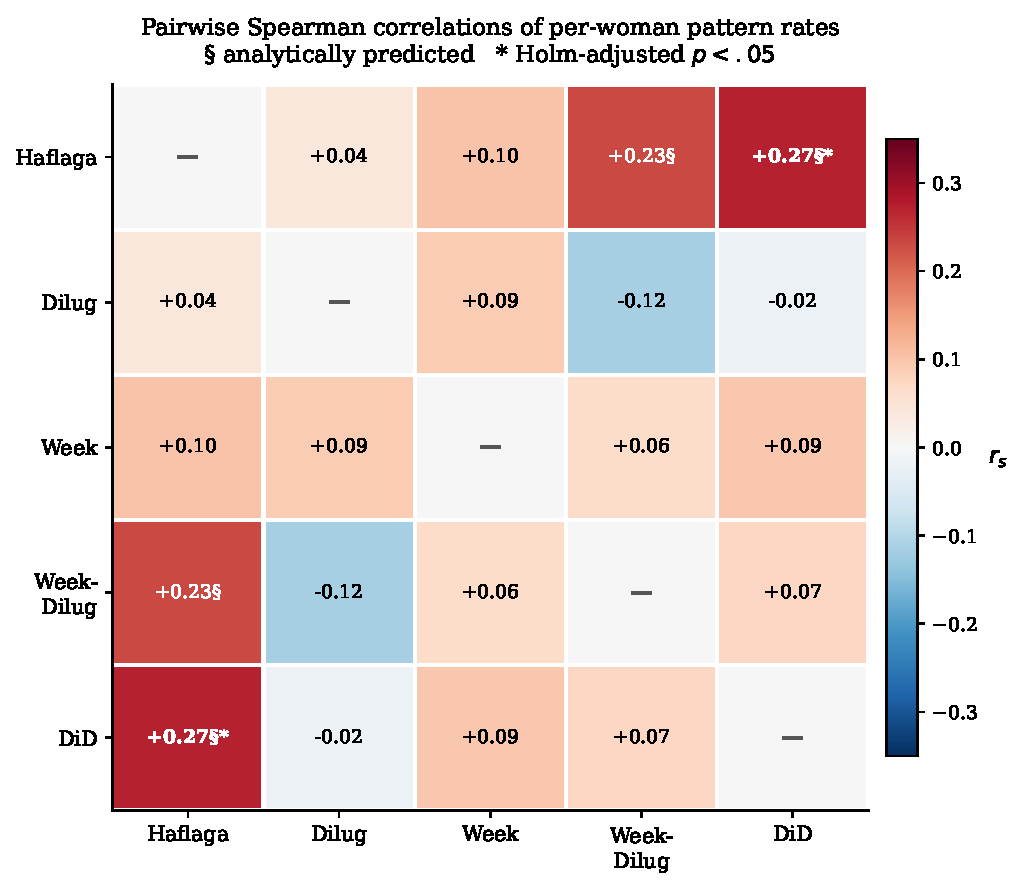
\includegraphics[width=0.8\textwidth]{fig8_chisq_heatmap}
  \caption{Spearman correlations between per-woman pattern rates. \S: analytically
    expected positive pair; *: Holm-adjusted $p < .05$. All pairwise tests are
    exploratory.}
  \label{fig:si-heatmap}
\end{figure}

\subsection*{S1.4 Robustness to follow-up length}

Because both rates in a pair can depend on follow-up, the unrestricted permutation tests
marginal rather than follow-up-conditional independence. Two checks, computed by the same
script with the same seed, bound the consequence for the two structurally expected pairs.
First, the partial Spearman correlation given $n_i$ (correlation of the rank residuals
after regressing each rank vector on the rank of $n_i$) is $0.254$ for Haflaga $\times$
Dilug-in-Dilug (unadjusted $0.269$) and $0.239$ for Haflaga $\times$ Week-Dilug
(unadjusted $0.231$). Second, restricting the $50{,}000$ permutations to exchange rates
only among women in the same follow-up quintile (strata of 24, 8, 31, 27 and 28 women)
preserves each rate's dependence on $n_i$ while breaking the association between
patterns; the resulting two-sided $p$-values are $.0046$ for Haflaga $\times$
Dilug-in-Dilug (unrestricted $.0036$) and $.0097$ for Haflaga $\times$ Week-Dilug
(unrestricted $.0113$). The exploratory conclusions are therefore not an artefact of
unequal follow-up. These checks are reported as robustness diagnostics for an
exploratory analysis, not as an additional primary result.

\subsection*{S1.5 Interpretation}

Three cautions apply. The associations are between women, not within sequences, and say
nothing about temporal ordering. They involve rare patterns (18 Week-Dilug and 27
Dilug-in-Dilug events) and rest on few women. And the surviving association is compatible
with the proximity argument but is not evidence for it: attributing co-occurrence to a
mechanism would require an explicit generative model for the sequences, which the article
does not fit.

\section{Literature Search for Prior Randomisation-Based Tests}
\label{sec:si-litsearch}

The main article states that we are not aware of any formal randomisation-based test of
whether the frequency of vesset-type arithmetic patterns in empirical cycle data departs
from a chance null. A hit was taken to contradict this only if it used empirical cycle
data, defined rule-based arithmetic events (equal intervals, constant first or second
differences, weekly anchors or equivalent) and compared their observed frequency with a
randomisation, permutation, bootstrap or Monte Carlo null. Descriptive halachic studies,
forecasting models, Markov models and regularity statistics were not counted.

The search had two stages. First, an unstructured search of the Hebrew and English
halachic, medical-halachic and biostatistical literatures carried out by the author while
preparing the dissertation (2019--2022); the quantitative halachic works it located are
cited in Section~2.3 of the main article and none tests pattern frequencies against a
randomisation null. Second, a logged web search on 16 September 2026 of twelve queries in
English and Hebrew combining the halachic terms (\textit{vesset}, \textit{veset},
\textit{haflaga}, \textit{dilug}, \textit{onah}, \textit{niddah}) with statistical
terms (permutation, randomisation, Monte Carlo, probability, empirical data), together
with citation-chasing queries for the author's earlier articles and for re-analyses of the
Marquette dataset. Every returned item was screened by title and snippet. No publication
meeting the criterion was found in either stage. The verbatim queries, hit descriptions
and limitations of the search (general web index rather than bibliographic databases;
snippet-level screening; possible unindexed Hebrew material) are recorded in
\texttt{revision\_reports/literature\_search\_log.md} in the code repository. The
main article therefore retains the wording ``we are not aware of'' rather than asserting
absence.

\section{The Zero-Count Rule \textit{Haflaga Chozer Chalila} Under the Three Nulls}
\label{sec:si-hcc}

\paragraph{Definition.} \textit{Haflaga Chozer Chalila} (``recurring haflaga'') is
established when a block of $m \geq 3$ consecutive haflaga values is repeated exactly,
three times in succession, so that the event occupies a window of $3m \geq 9$ cycles.
Thus $(25, 27, 26, 25, 27, 26, 25, 27, 26)$ is an event, $(25, 27, 26, 28)$ repeated three
times is an event with $m = 4$, and $(25, 27, 25, 27, 25, 27)$ is not (block of length 2).
It is the sixth and last rule computable from interval lengths alone; the other
repeating rule of the halachic literature, \textit{Dilug Chozer Chalila}, depends on
calendar dates and is not computable from these data.

\paragraph{Counting convention.} As for the five primary rules, distinct maximal
$m$-periodic segments of length at least $3m$ count once each. A segment whose block has
a shorter period $d$ dividing $m$ is not counted at $m$: it is the same event at period
$d$ if $d \geq 3$, a Haflaga if $d = 1$, and not an event if $d = 2$. The rule is
implemented twice (a reference loop and a vectorised version) in
\texttt{scripts/hcc\_rule.py}, and the two implementations agree on the observed data and
on 3,000 random sequences with planted repeating blocks. In the observed data 100 of the
118 women have the nine or more cycles needed for an event; the observed count is 0.

\paragraph{Null distributions.} The rule was counted under $\HG$, $\HI$ and $\HW$
with $B = 50{,}000$ replicates each (seed 17), using the same generators as the main
analysis (Table~\ref{tab:si-hcc}). Under the two global nulls an event occurs in fewer
than 1 in 2,000 replicates; under $\HW$, which preserves each woman's multiset of
values, a periodic reordering of a woman with few distinct values and many cycles is
occasionally produced, and at least one event occurs in 2.8\% of replicates. The
observed zero is the modal outcome under every null and its two-sided Monte Carlo
$p$-value is 1. The replicate counts are stored in \texttt{results/hcc\_null.npz}.

\paragraph{Effect on the joint statistic.} Because a near-degenerate component could in
principle disturb the estimated covariance of the joint test, the check was made
directly. The three null streams were regenerated with the seed and call order of the
main analysis, so that the five primary counts reproduce the stored replicates exactly,
and the rule was counted on the same permuted sequences, giving paired six-component
replicate vectors (\texttt{scripts/hcc\_joint.py}; \texttt{results/hcc\_joint.npz}).
Table~\ref{tab:si-hcc-joint} compares the five- and six-component Mahalanobis tests.
The observed $D_M$ is unchanged to two decimals under every null, because the observed
deviation of the sixth component from its null mean is essentially zero. The $p$-values
increase slightly: every replicate that contains an event lies far beyond the observed
vector in the sixth coordinate, so such replicates are added to the exceedance count
(16, 19 and 1,378 replicates under $\HG$, $\HI$ and $\HW$). The split-batch estimate
agrees. Under the two global nulls the joint test still rejects at $p < .001$; under
$\HW$ the $p$-value moves from $.126$ to $.150$ and the test still does not reject. The
condition numbers of the estimated $6 \times 6$ covariance matrices ($1.4 \times 10^5$,
$1.2 \times 10^5$ and $2.0 \times 10^3$) reflect the near-zero variance of the sixth
component but caused no numerical difficulty.

\begin{table}[!htbp]
\centering
\caption{Joint Mahalanobis test with five components (main article) and with
  \textit{Haflaga Chozer Chalila} added as a sixth component, on the same $B = 50{,}000$
  paired replicates per null.}
\label{tab:si-hcc-joint}
\smallskip
\begin{tabular}{L{1.4cm} C{1.4cm} C{1.6cm} C{1.4cm} C{1.6cm} C{2.6cm}}
\toprule
\textbf{Null} & $\mathbf{D_M^{(5)}}$ & $\mathbf{p^{(5)}}$ & $\mathbf{D_M^{(6)}}$ & $\mathbf{p^{(6)}}$ & \textbf{Split-batch} $\mathbf{D_M^{(6)}}$, $\mathbf{p^{(6)}}$ \\
\midrule
$\HG$  & 5.08 & $.0001$ & 5.08 & $.0005$ & 5.07, $.0005$ \\
$\HI$  & 4.87 & $.0004$ & 4.87 & $.0007$ & 4.87, $.0007$ \\
$\HW$  & 2.93 & $.126$  & 2.94 & $.150$  & 2.96, $.143$ \\
\bottomrule
\end{tabular}
\end{table}

\begin{table}[!htbp]
\centering
\caption{\textit{Haflaga Chozer Chalila} under the three nulls ($B = 50{,}000$ each;
  observed count 0).}
\label{tab:si-hcc}
\smallskip
\begin{tabular}{L{2.2cm} C{1.6cm} C{1.6cm} C{1.6cm} C{2.6cm} C{2.0cm}}
\toprule
\textbf{Null} & \textbf{Mean} & \textbf{SD} & \textbf{Max} & \textbf{P(count $\geq 1$)} & \textbf{$p$ (two-sided)} \\
\midrule
$\HG$   & 0.0003 & 0.018 & 1 & 0.0003 & 1.00 \\
$\HI$   & 0.0004 & 0.020 & 1 & 0.0004 & 1.00 \\
$\HW$   & 0.028  & 0.166 & 2 & 0.028  & 1.00 \\
\bottomrule
\end{tabular}
\end{table}

\end{document}
